\chapter{First Real Chapter} \label{sample chapter}

I am sorry, this is only a sample chapter so it really has no point except to show you what a chapter looks like in this document style. You should not bother to read all of this, there is no useful information to be found here. Or is there? Have you noticed that \LaTeX\ automatically fixed references for you? The hyperref package, which is activated by default in this thesis class, even creates fancy clickable references, like this one: \reffig{sample figure}.

If you run into any problems with \LaTeX, you might want to take a look at \textit{The Not So Short Introduction to \LaTeX2e}, by Tobias Oetiker. You can find it at the following location: \url{http://tobi.oetiker.ch/lshort/lshort.pdf}.

\section{Advantages}

A strong point is the beautiful way \LaTeX\ typesets math equations. Take a look at the identity, made famous by Euler himself:
\begin{equation}
e^{j\pi} + 1 = 0.
\end{equation}
This is a beautiful equation on its own, but my point is that \LaTeX\ really enables you to easily create equations that look nice and readable.

\section{Disadvantages}

Getting started with \LaTeX\ can be difficult and confusing. Especially the way you add illustrations to your document is awkward. This thesis uses vector-based EPS illustrations, which always look crisp when printed.

However, sometimes you also need to use bitmap pictures like JPG or PNG. Unfortunately you can not use both vector graphics and bitmap graphics in the same document. You actually need a different compiler to process \LaTeX\ with, like pdf\LaTeX. You might want to try and convert you JPGs to EPS using \texttt{xv}, \texttt{convert} or \texttt{jpeg2eps}. The photograph in \reffig{FIG RTG} was converted using \texttt{jpeg2eps}.

Getting started with \LaTeX\ can be difficult and confusing. Especially the way you add illustrations to your document is awkward. This thesis uses vector-based EPS illustrations, which always look crisp when printed.

Getting started with \LaTeX\ can be difficult and confusing. Especially the way you add illustrations to your document is awkward. This thesis uses vector-based EPS illustrations, which always look crisp when printed.

Getting started with \LaTeX\ can be difficult and confusing. Especially the way you add illustrations to your document is awkward. This thesis uses vector-based EPS illustrations, which always look crisp when printed.

\begin{figure}%
\centering%
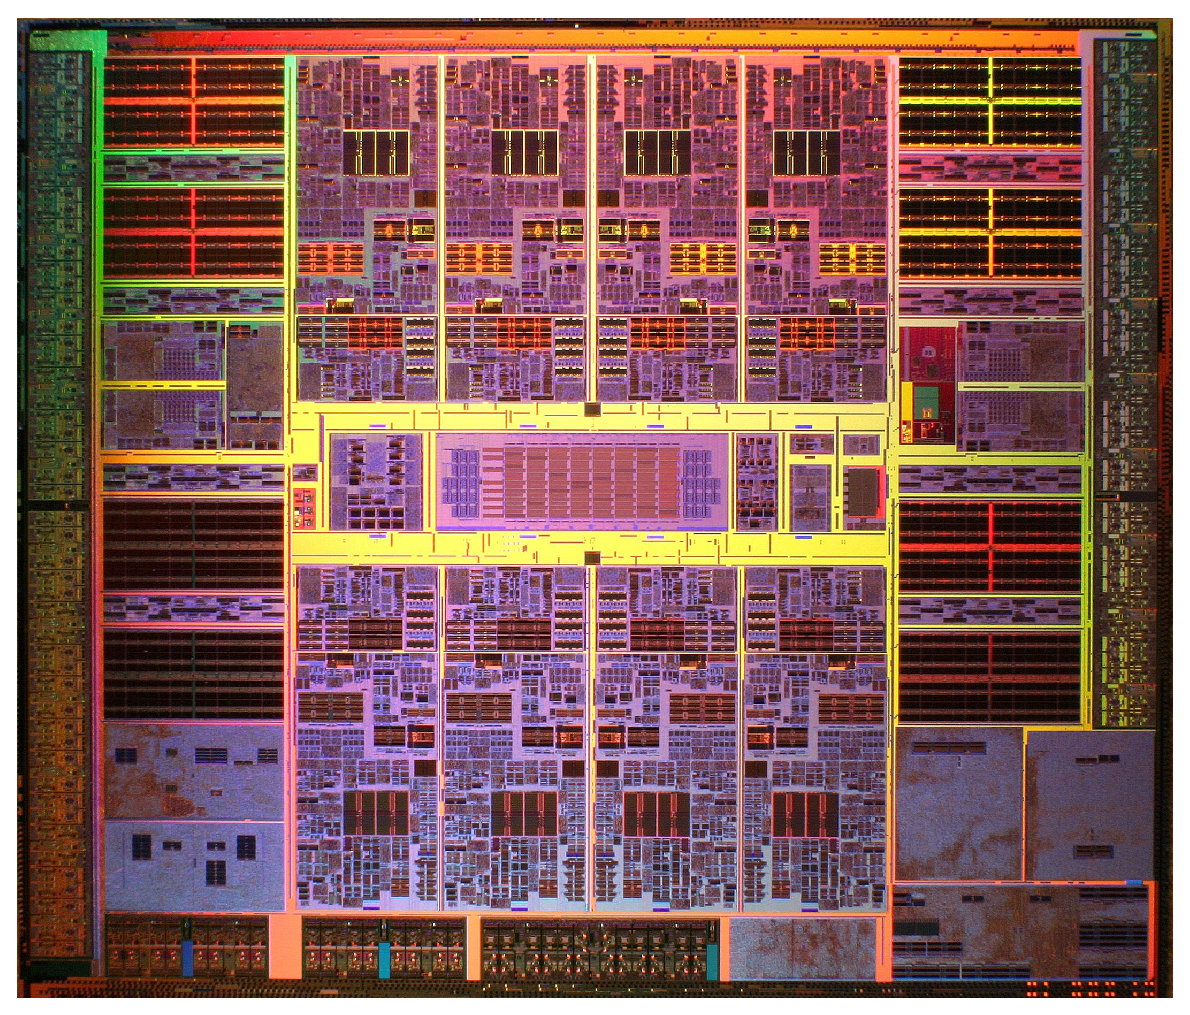
\includegraphics[width=.7\textwidth]{demopic}%
\caption{UltraSparc T2 microprocessor}%
\label{FIG RTG}%
\end{figure} 